\documentclass[a4paper,14pt]{extreport}
  \usepackage[left=1.5cm,right=1.5cm,
      top=1.5cm,bottom=2cm,bindingoffset=0cm]{geometry}
  \usepackage{scrextend}
  \usepackage[T1,T2A]{fontenc}
  \usepackage[utf8]{inputenc}
  \usepackage[english,russian,ukrainian]{babel}
  \usepackage{tabularx}
  \usepackage{amssymb}
  \usepackage{color}
  \usepackage{amsmath}
  \usepackage{mathrsfs}
  \usepackage{listings}
  \usepackage{graphicx}
  \usepackage{xcolor}
  \usepackage{hyperref}

  



  
  
%}

\newcommand{\img}[4]{\center{\includegraphics[width=#1\linewidth]{#2}}\captionof{figure}{#3}\label{#4}}
\begin{document}
  \pagecolor{white}

  %----------------------------------------1
\begin{titlepage}
    \begin{center}
    \large
    Національний технічний університет України \\ "Київський політехнічний інститут імені Ігоря Сікорського"


    Факультет Електроніки

    Кафедра мікроелектроніки
    \vfill

    \textsc{ЗВІТ}\\

    {\Large Про виконання лабораторної роботи №5\\
    з дисципліни: «Мікропроцесори та мікроконтролери»\\[1cm]

    %Резистивні сенсори температури


    }
    \bigskip
    \end{center}
    \vfill

    \newlength{\ML}
    \settowidth{\ML}{«\underline{\hspace{0.4cm}}» \underline{\hspace{2cm}}}
    \hfill
    \begin{minipage}{1\textwidth}
    Виконавець:\\
    Студент 4-го курсу \hspace{4cm} $\underset{\text{(підпис)}}{\underline{\hspace{0.2\textwidth}}}$  \hspace{1cm}А.\,С.~Мнацаканов\\
    \vspace{1cm}

    Перевірив: \hspace{6.1cm} $\underset{\text{(підпис)}}{\underline{\hspace{0.2\textwidth}}}$  \hspace{1cm} Татарчук Д. Д.\\

    \end{minipage}

    \vfill

    \begin{center}
    2021
    \end{center}
\end{titlepage}



\newpage
\setcounter{page}{2}


\begin{center}
\begin{figure}
\center{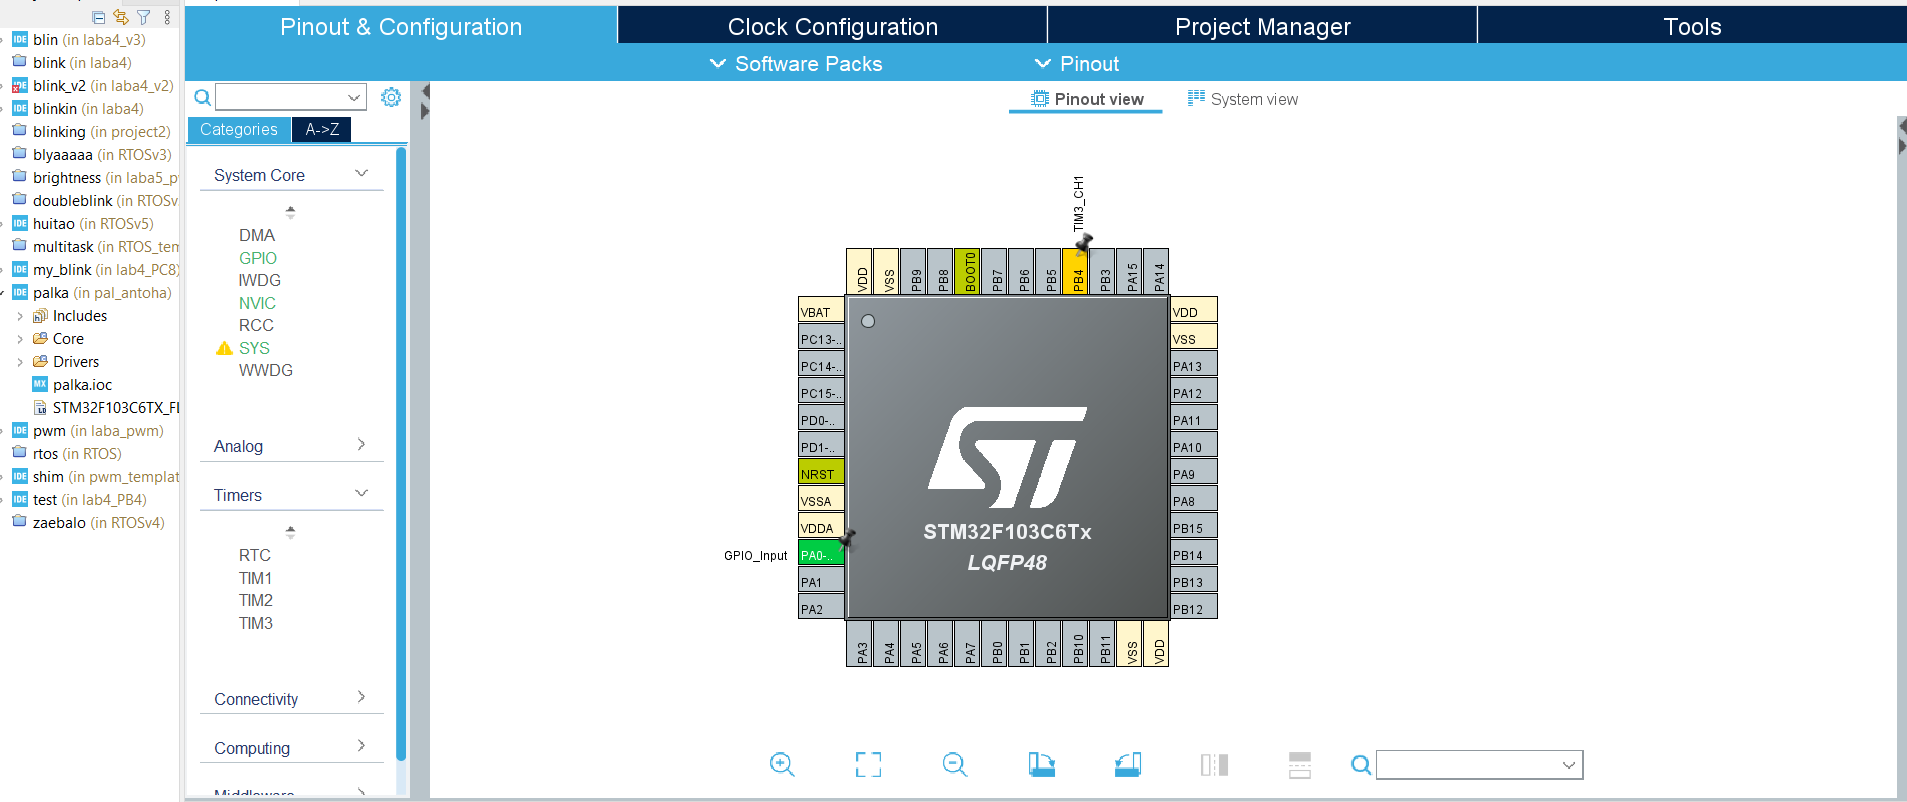
\includegraphics[width=0.7\linewidth]{1.png}
\caption{Налагодження ніжок мікроконтролера}}
\end{figure}
\end{center}

\begin{center}
КОД
\end{center}

\begin{verbatim}  
 
  int coef_fill = 0;  
 
  int but_prev = 0;
  int but_cur = 0;
 
  int a = 0;  
  /* USER CODE END PV */
  /* USER CODE BEGIN 2 */
  HAL_TIM_Base_Start (& htim3 ) ;  
  HAL_TIM_PWM_Init (& htim3 ) ;  
  HAL_TIM_PWM_Start (& htim3 , TIM_CHANNEL_1 ) ;
  HAL_TIM_Base_Start_IT (& htim3 ) ;  
  /* USER CODE END 2 */
  /* USER CODE BEGIN 0 */

  void HAL_TIM_PeriodElapsedCallback( TIM_HandleTypeDef * htim )
  {
  if( htim - > Instance == TIM3 ) 
  {
  htim3 . Instance - > CCR1 = coef_fill ; 
  }
  }
  /* USER CODE END 0 */
  
  while (1)
  {
  if ( a ==19)
  {
  coef_fill = 0;
  a = 0;
  }
 
  else
  {
  but_cur = HAL_GPIO_ReadPin ( GPIOA , GPIO_PIN_0 ) ;
 
  if ( ( but_prev == 0) && ( but_cur != 0) )
  {
  coef_fill +=50;
  a += 1;
  }
 
 else
  {
  coef_fill = coef_fill ;
 }
 
  but_prev = but_cur ;
  }
  }

\end{verbatim}



\begin{center}
Результат
\end{center}

Написана програму, в якiй по натисканню кнопки змiнюється яскравiсть зеленого свiтлодiоду.



\end{document}